\subsection{UC-9}
\label{subsec:UC-9}


\begin{figure}[H]
    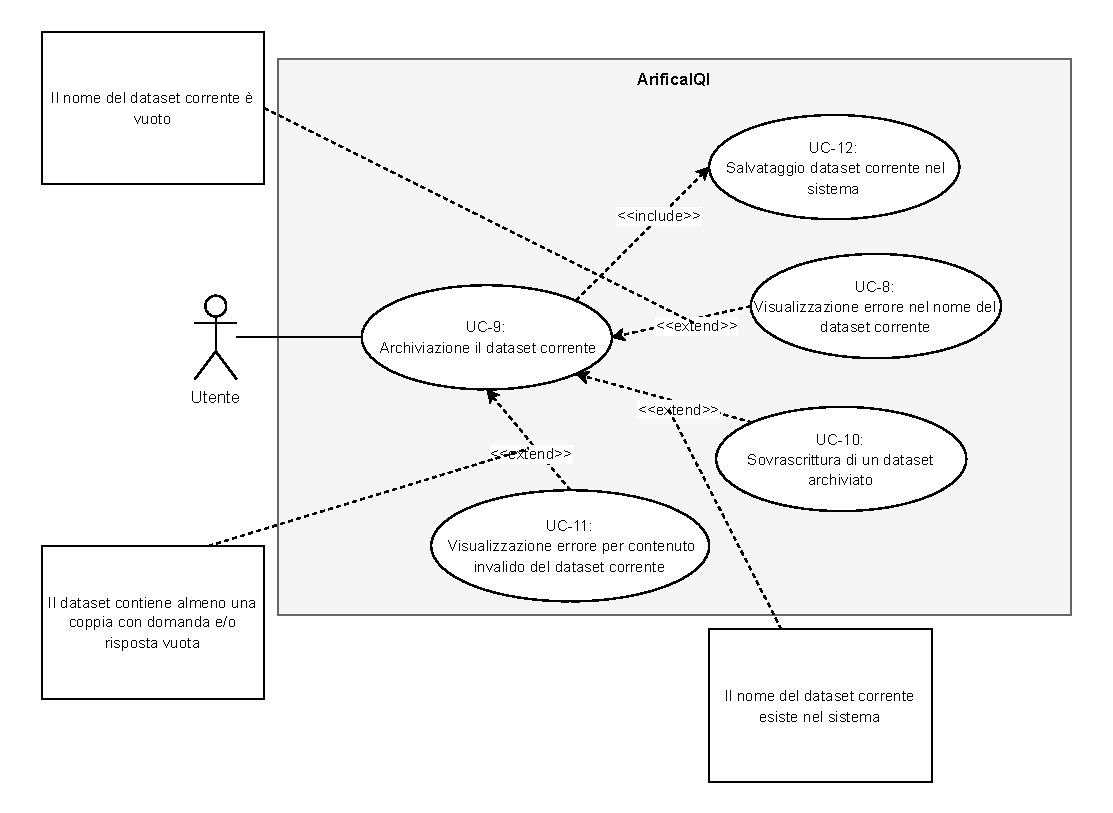
\includegraphics[scale=0.75]{Sezioni/UseCase/Immagini/UC-9.pdf}
    \caption{Diagramma UC-9.}
\end{figure}

\begin{usecase}{UC-9}{Archiviazione del dataset corrente}
    
    \req{\hyperref[item:RU-3]{RU-3}} 

    \pre{
        \item Il sistema è attivo e funzionante
        \item Il dataset corrente non è vuoto
    }

    \post{
        \item Il dataset corrente viene archiviato nel sistema
    }
    
    \actor{Utente}

    \subactors{}

    \trigger{L'utente deve archiviare il dataset corrente per renderlo persistente}
    
    \inc{\hyperref[subsec:UC-12]{UC-12}}

    \base{}

    \scenario{
        \item L'utente richiede l'archiviazione del dataset corrente.
        \item \texttt{<<include:UC-12>>}
    }

    \subscenario{
        \item[1.1] \textbf{Il nome del dataset corrente è vuoto}
        \begin{itemize}
            \item [a.] \hyperref[subsec:UC-8]{UC-8}
        \end{itemize}
        \item[1.2]\textbf{Esiste già un dataset archiviato nel sistema con nome uguale al dataset corrente}
        \begin{itemize}
            \item[a.] \hyperref[subsec:UC-10]{UC-10}
        \end{itemize}
        \item[1.3] \textbf{Il dataset contiene almeno una coppia con domanda e/o risposta vuota}
        \begin{itemize}
            \item[a.] \hyperref[subsec:UC-11]{UC-11}
        \end{itemize}
    }
\end{usecase}
